\documentclass[crop, tikz]{standalone}

\usepackage[utf8]{inputenc}
% 'crop' is the default for v1.0, before it was 'preview'
%\usetikzlibrary{...}% tikz package already loaded by 'tikz' option

\usetikzlibrary{arrows}
\usetikzlibrary{decorations.markings}

\begin{document}

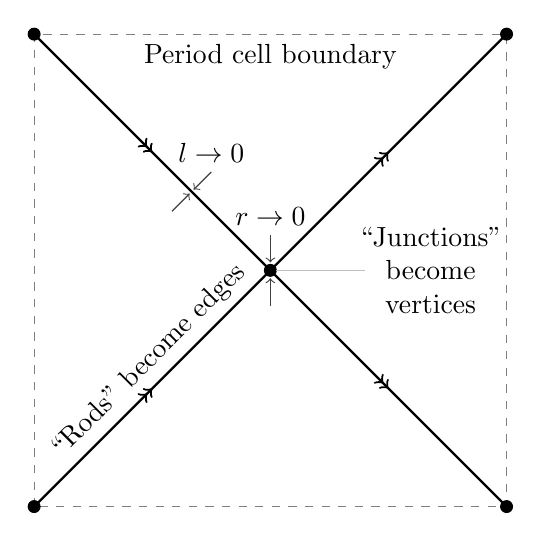
\begin{tikzpicture}

	%period cell boundary	
	\draw[dashed, black!50!white] (-3,-3) rectangle (3,3);
	\node[anchor=north] at (0,3) {Period cell boundary};

	%edges
	\begin{scope}[decoration={markings, mark=at position 0.5 with {\arrow{>>}}}]
		\draw[postaction={decorate}, thick] (-3,-3) -- (0,0);
		\draw[postaction={decorate}, thick] (0,0) -- (3,3);
		\draw[postaction={decorate}, thick] (-3,3) -- (0,0);
		\draw[postaction={decorate}, thick] (0,0) -- (3,-3);
	\end{scope}

	%vertices
	\filldraw[black] (0,0) circle (0.075);
	\filldraw[black] (-3,-3) circle (0.075);
	\filldraw[black] (-3,3) circle (0.075);
	\filldraw[black] (3,3) circle (0.075);
	\filldraw[black] (3,-3) circle (0.075);

	%labels
	\node[anchor=south, rotate=45] at (-1.35,-1.35) {``Rods" become edges};
	\node[anchor=west, align=center] at (1,0) {``Junctions" \\ become \\ vertices};
	\draw[black!25!white] (1+0.2,0) -- (0 + 0.075,0);

	%limits
	\draw[->, black!75!white] (-1 - 0.25, 1 - 0.25) -- (-1 - 0.025, 1 - 0.025);
	\draw[->, black!75!white] (-1 + 0.25, 1 + 0.25) -- (-1 + 0.025, 1 + 0.025);
	\node[anchor=south] at (-1 + 0.25, 1 + 0.25) {$l\rightarrow 0$};

	\draw[->, black!75!white] (0, -0.45) -- (0, -0.1);
	\draw[->, black!75!white] (0, 0.45) -- (0, 0.1);
	\node[anchor=south] at (0, 0.45) {$r\rightarrow0$};

\end{tikzpicture}

\end{document}